\documentclass{article}
\usepackage{tikz}
\usetikzlibrary{positioning}

\begin{document}

\begin{figure}[h]
    \centering
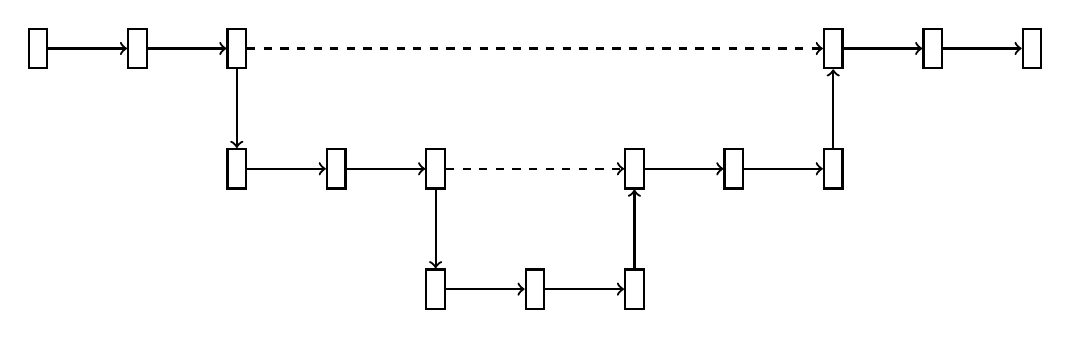
\begin{tikzpicture}[node distance=1cm, auto, thick]

    % Define styles
    \tikzstyle{rec} = [draw, rectangle, minimum width=0.2cm, minimum height=0.5cm]

    % ENCODER
    \node (en1_input) [rec] {};
    \node (en1con1_output) [rec, right=of en1_input] {};
    \node (en1con2_output) [rec, right=of en1con1_output] {};

    \node (en2_input) [rec, below=of en1con2_output] {};
    \node (en2con1_output) [rec, right=of en2_input] {};
    \node (en2con2_output) [rec, right=of en2con1_output] {};

    \node (en3_input) [rec, below=of en2con2_output] {};
    \node (en3con1_output) [rec, right=of en3_input] {};
    \node (en3con2_output) [rec, right=of en3con1_output] {};

    % DECODER
    \node (de1_input) [rec, above=of en3con2_output] {};
    \node (de1con1_output) [rec, right=of de1_input] {};
    \node (de1con2_output) [rec, right=of de1con1_output] {};

    \node (de2_input) [rec, above=of de1con2_output] {};
    \node (de2con1_output) [rec, right=of de2_input] {};
    \node (de2con2_output) [rec, right=of de2con1_output] {};

    % CONNECTIONS
    \draw[->] (en1_input) -- (en1con1_output);
    \draw[->] (en1con1_output) -- (en1con2_output);
    \draw[->] (en1con2_output) -- ++(0,-0.5) -| (en2_input);
    \draw[->] (en2_input) -- (en2con1_output);
    \draw[->] (en2con1_output) -- (en2con2_output);
    \draw[->] (en2con2_output) -- ++(0,-0.5) -| (en3_input);
    \draw[->] (en3_input) -- (en3con1_output);
    \draw[->] (en3con1_output) -- (en3con2_output);
    \draw[->] (en3con2_output) -- ++(0,0.5) -| (de1_input);
    \draw[->] (de1_input) -- (de1con1_output);
    \draw[->] (de1con1_output) -- (de1con2_output);
    \draw[->] (de1con2_output) -- ++(0,0.5) -| (de2_input);
    \draw[->] (de2_input) -- (de2con1_output);
    \draw[->] (de2con1_output) -- (de2con2_output);

    % Skip connections
    \draw[->, dashed] (en2con2_output.east) -- ++(0.5,0) |- (de1_input.west);
    \draw[->, dashed] (en1con2_output.east) -- ++(0.5,0) |- (de2_input.west);

\end{tikzpicture}
\caption{U-Net Architecture Diagram}
\end{figure}

\end{document}
